% main.tex -- draft manuscript, prepared by claude-interactive.11 (claude-opus-5-5, claude), 2026-10-18,
% task T-20261018-claude-interactive.11-01. Build with ./build.sh. Every number cites a run id under runs/
% (figure captions, text and the provenance table of Appendix G).
\documentclass[aps,pra,twocolumn,superscriptaddress,nofootinbib,floatfix]{revtex4-2}
\usepackage[T1]{fontenc}
\usepackage{amsmath}
\usepackage{newtxtext,newtxmath}
\usepackage{graphicx}
\usepackage{xcolor}
\usepackage[colorlinks=true,linkcolor={blue!45!black},citecolor={blue!45!black},urlcolor={blue!45!black}]{hyperref}
\usepackage{xurl}
\hypersetup{pdftitle={Statistics of Kerr-thermalized light in multimode fibre},
  pdfauthor={Authors to be set by the PI; draft by claude-interactive.11 (Claude Opus 5.5)}}

\newcommand{\LNL}{L_{\rm NL}}
\newcommand{\smax}{\sigma_{\max}}
\DeclareRobustCommand{\run}[1]{{\small\path{#1}}}
\newcommand{\ekn}{E'/\kappa N}

\begin{document}

\title{Statistics of Kerr-thermalized light in multimode fibre:\\
exact Dirichlet mode statistics and the limits of squeezing}

\author{Authors: to be set by the PI}
\noaffiliation

\date{Draft, October 18, 2026}

\begin{abstract}
Kerr nonlinearity drives the modal powers of light in a graded-index multimode fibre towards a Rayleigh--Jeans
distribution and, at low energy, condenses power into the fundamental mode. Beyond the mean occupations, we collect
analytical results on the fluctuations and quantum noise of this light, each checked by an independent simulation written
by a second model family. (i) When the excitation energy per unit power is
below the first modal gap, the microcanonical Rayleigh--Jeans state has exactly Dirichlet-distributed scaled excitation
powers at any mode number $M$: every excited mode has $g^{(2)}=2-2/M$, and the condensate--mode covariance changes sign
at the harmonic mean of the excitation energies. (ii) Before the quantum state scrambles, the multimode quadrature
squeezing of a coherent launch is $\sigma_{\max}^{-2}$, from the classical tangent map, only while
$\sigma_{\max}^6/n_0\lesssim1$; the curvature of the Kerr crescent sets the leading correction. (iii) The condensate's
own squeezing is $\lambda_-\simeq\det V/V_P$, with a computable error; it is about $-9.5$~dB at ten nonlinear lengths in a
15-mode model. (iv) On its early shear branch a Kerr stage squeezes a displaced thermal state of mixedness $\nu$
at best to $\frac{3}{2\cdot4^{1/3}}(\nu^4/n_d)^{1/3}$, and cannot squeeze a phase-invariant state at all. We state each regime, what failed in verification, and what to measure.
\end{abstract}

\maketitle

%=====================================================================================================
\section{Introduction}

Kerr nonlinearity in a graded-index (GRIN) multimode fibre redistributes power among the guided modes, and the modal
powers relax towards a Rayleigh--Jeans (RJ) distribution. At low energy, power condenses into the fundamental mode,
which is one account of beam self-cleaning~\cite{picozzi2014,baudin2020,pourbeyram2022,baudin2023}. Weak random coupling within degenerate groups accelerates the
relaxation~\cite{fusaro2019,garnier2019}; strong coupling between groups competes with it~\cite{berti2022}. Wave-turbulence theory~\cite{picozzi2014,connaughton2005,aschieri2011}
and its quantum extensions~\cite{chiocchetta2016,zanaglia2025} predict the mean occupations, and experiments measure
them by averaging over pulses or speckle realizations~\cite{pourbeyram2022,baudin2020,baudin2023}.

This paper concerns what the means leave out: the fluctuations of the modal powers in the thermalized state
(Sec.~\ref{sec:dir}), the quantum noise of the light early in the propagation, before its quantum state scrambles
(Secs.~\ref{sec:early} and \ref{sec:own}), and the squeezing of the condensate after it leaves the fibre
(Sec.~\ref{sec:stage}). For each result we give the steps that carry the derivation, the regime as bounds on
dimensionless groups, and how it was checked.

Each result was proposed by one model family (Claude) and checked by an independent implementation written by another
(GPT), against predictions frozen before the runs; several original statements failed and were narrowed. None is
formalized or peer reviewed. Table~\ref{tab:status} gives the status; the Appendices give full derivations and the
run and verifying agent of every number.

We build on known results: finite-mode microcanonical departures from RJ in bosonic oligomers~\cite{vardi2024};
classical-field condensate statistics in the canonical ensemble~\cite{witkowska2009}; canonical versus microcanonical
condensate fluctuations~\cite{holthaus1998}; the coherent-state Kerr optimum
$0.945\,n^{-1/3}$ at fixed photon number~\cite{najafabadi2023} (ingredients in Ref.~\cite{bajer2002}); the Kerr crescent and interferometric number squeezing~\cite{kitagawa1986}
and one-axis twisting~\cite{kitagawa1993}; the invariance of phase-averaged states under Kerr
evolution~\cite{vintskevich2019}; and linearized propagation of multimode quantum noise in fibres~\cite{sloan2025}.
A conference abstract reports entanglement arising during thermalization~\cite{birk2023}; we have not seen a full
paper. Bounded literature searches did not find the Dirichlet law and its covariance structure for condensed RJ light,
the curvature bound on multimode squeezing in a thermalizing fibre, or the mixedness factor $\nu^{4/3}$; these searches
do not establish novelty.

%=====================================================================================================
\section{Model and scales}\label{sec:model}

We use a scalar field in one polarization, with modal amplitudes $A_p(z)$, $p=0,\dots,M-1$, normalized so that
$I_p=|A_p|^2$ is the modal power:
\begin{equation}
i\partial_zA_p=\varepsilon_pA_p-\gamma\textstyle\sum_{qrs}S_{pqrs}A_q^*A_rA_s .\label{eq:nlse}
\end{equation}
Here $\varepsilon_p\ge0$ is the propagation-constant offset from the fundamental ($\varepsilon_0=0$), $S_{pqrs}$ the
real, symmetric Kerr overlap and $\gamma$ the nonlinear coefficient. A parabolic index profile gives $K$ equidistant
groups, $\varepsilon=q\kappa$ with $q=0,\dots,K-1$ and degeneracy $q+1$, so $M=K(K+1)/2$. When the Kerr energy is small
against the gap, $L_{\rm beat}/\LNL\ll1$ with $\LNL=1/(\gamma N)$ and $N$ the total power, averaging over the beat length leaves a resonant normal
form~\cite{podivilov2019} that conserves the power $N=\sum_pI_p$, the excitation energy $E'=\sum_p\varepsilon_pI_p$ and
the resonant Kerr energy $H_{\rm res}$. Real fibres have weak random linear coupling among degenerate modes~\cite{fusaro2019,garnier2019}; it conserves $N$
and $E'$ but not $H_{\rm res}$ or the orbital angular momentum $L_z$. For the scalar model we take Hermitian Brownian
coupling of amplitude $\sigma$ within each degenerate spatial group (the cited works couple polarizations), with
decorrelation length $L_d=\LNL/\sigma^2$.

For quantum noise we quantize each temporal coherence cell of duration $\tau$ separately, neglecting the coupling of cells
by dispersion and walk-off: $[a_p,a_q^\dagger]=\delta_{pq}$ and $n=N\tau/\hbar\omega$ photons per cell (for example
$n\approx5\times10^{10}$ for 10~kW in 1~ps at 1~$\mu$m). The mean evolution depends only on $\gamma N$; quantum
fluctuations enter through $1/n$. Quadratures $X_\theta=ae^{-i\theta}+a^\dagger e^{i\theta}$ have vacuum variance 1.
The fundamental holds $n_0=f_0n$ photons.

The dimensionless groups are the scaled energy $\ekn$ (equivalently the condensate fraction $f_0$), the mode number $M$
(or $K$), $L_d/\LNL$, $z/\LNL$, $n$ and $L_{\rm beat}/\LNL$. The cross-family checks used an independent implementation of
the resonant model with exact Hermite--Gauss overlaps, $K=4$--6 ($M=10$--21), tangent-map and truncated-Wigner (TWA)
propagation, and exact one- and three-mode quantum references (Appendix~\ref{app:methods}).

%=====================================================================================================
\section{Dirichlet statistics of the condensed RJ state}\label{sec:dir}

\textit{Statement.} Suppose that the only conserved quantities of the modal powers are $N$ and $E'$, and that the
statistics are those of the flat (Liouville) measure on that shell. Let $D=M-1$ be the number of excited modes and
$\kappa=\min_{m\ge1}\varepsilon_m$ the first gap. If
\begin{equation}
0<E'\le\kappa N, \label{eq:cond}
\end{equation}
that is, if the excitation energy per unit power lies below the first gap, the scaled excitation powers
$x_m=\varepsilon_mI_m/E'$ ($m=1,\dots,D$) are exactly uniform on the simplex $\sum_mx_m=1$: $x\sim{\rm Dirichlet}(1,\dots,1)$,
with $I_0=N-\sum_mI_m$.

\textit{Crux.} Write $A_p=\sqrt{I_p}\,e^{i\phi_p}$. Because $d^2A_p=\tfrac12dI_p\,d\phi_p$, the measure
$\delta(\sum I-N)\,\delta(\sum\varepsilon I-E')\prod_pd^2A_p$ is flat in the intensities on the polytope
$\{I\ge0,\ \sum I=N,\ \sum\varepsilon I=E'\}$. Integrating out $I_0$ with the first delta function leaves only the
condition $I_0\ge0$, i.e.\ $\sum_mI_m\le N$. Under Eq.~\eqref{eq:cond} this condition cannot bind, since
$\sum_mI_m\le\sum_m(\varepsilon_m/\kappa)I_m=E'/\kappa\le N$: the condensate absorbs or supplies power at no energy cost.
What remains is one linear constraint on $D$ nonnegative variables, and the rescaling to $x_m$ has a constant Jacobian.
No large-$M$ or small-depletion expansion enters.

\textit{Consequences.} The Dirichlet moments $\langle x_m\rangle=1/D$, $\langle x_m^2\rangle=2/[D(D+1)]$ and
$\langle x_mx_n\rangle=1/[D(D+1)]$ ($m\ne n$) give, with $S_r=\sum_{m\ge1}\varepsilon_m^{-r}$,
\begin{gather}
\langle I_m\rangle=\frac{E'}{D\varepsilon_m},\quad g^{(2)}_m=2-\frac{2}{M},\quad g^{(2)}_{mn}=1-\frac1M,\label{eq:g2}\\
{\rm Var}\,I_0=\frac{E'^2(DS_2-S_1^2)}{D^2(D+1)},\label{eq:var}\\
{\rm Cov}(I_0,I_m)=-\frac{E'^2}{\varepsilon_m}\,\frac{D/\varepsilon_m-S_1}{D^2(D+1)} ,\label{eq:cov}
\end{gather}
where $g^{(2)}_m=\langle I_m^2\rangle/\langle I_m\rangle^2$. The means are RJ with the chemical potential at the
fundamental, exactly, at any $M$. Every excited mode has the same $g^{(2)}$, independent of its energy and of $E'$; it
falls short of the thermal value 2 by $2/M$, the trace of the fixed total energy. The condensate is anticorrelated with
modes below the harmonic mean $D/S_1$ of the excitation energies and correlated with modes above it. For the GRIN ladder,
$D=K(K+1)/2-1$, $\kappa S_1=K-1+H_{K-1}$ and $\kappa^2S_2=H_{K-1}+H^{(2)}_{K-1}$ (harmonic numbers), so the sign change
lies between groups 2 and 3 for $K=5$ and 6, and the depletion $N_{\rm ex}=N-I_0$ has
${\rm Var}\,N_{\rm ex}/\langle N_{\rm ex}\rangle^2\to(\ln K+\gamma_E+\pi^2/6-2)/K^2$ (Appendix~\ref{app:dirichlet}). The
single-mode law, Beta$(1,D-1)$, is the textbook energy law of one of $D$ oscillators at fixed total energy; what is new is
that the condensate maps the condensed RJ state exactly onto it. Above $E'=\kappa N$ the condition $I_0\ge0$ binds
(Appendix~\ref{app:dirichlet}).

\begin{figure}[t]
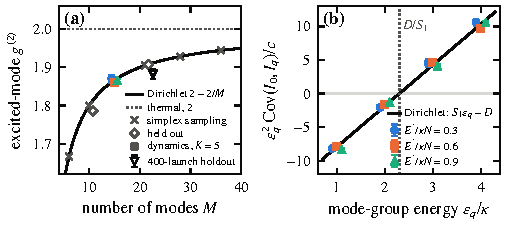
\includegraphics[width=\columnwidth]{figures/fig1_dirichlet.pdf}
\caption{Dirichlet statistics of condensed RJ light. (a) Excited-mode $g^{(2)}$ against mode number. Line:
Eq.~\eqref{eq:g2}. Crosses: sampling of the measure. Coloured symbols: dynamics at $K=5$, $L_d/\LNL=11.1$,
$z/\LNL\in[2000,8000]$, for $\ekn=0.3$ (circles), 0.6 (squares), 0.9 (triangles). Diamonds: held-out $K=4$, 6.
Down-triangle: fresh 400-launch holdout. Error bars: one standard error (SE) over disorder realizations. (b) Condensate--mode covariance for $K=5$, multiplied by
$\varepsilon_q^2/c$ with $c=E'^2/[D^2(D+1)]$, so that Eq.~\eqref{eq:cov} becomes the line $S_1\varepsilon_q-D$ ($\kappa=1$),
which crosses zero at $D/S_1=2.30\kappa$. Near the crossing relative errors are larger (30\% at $q=2$, $\ekn=0.9$); the
verified statement is the sign. Run: \run{2026-10-17-gpt-b-dirichlet}.}
\label{fig:dirichlet}
\end{figure}

\textit{Checks.} Independent sampling of the simplex for $M=6$--36 gives $2-g^{(2)}\propto M^{-1.0017\pm0.0021}$ with
coefficient $2.008\pm0.012$ (exact: 2). The dynamical tests used $L_d/\LNL=11.1$, the window $z/\LNL\in[2000,8000]$
and six launch and disorder realizations per case. At $K=5$ and $\ekn=0.3$, 0.6, 0.9 the pooled
excited-mode $g^{(2)}$ is 1.870, 1.859, 1.865 against $28/15=1.867$, and ${\rm Var}\,I_0$ is $1.03\pm0.02$, $0.99\pm0.04$
and $1.04\pm0.03$ times Eq.~\eqref{eq:var}; every resolved covariance sign agrees with Eq.~\eqref{eq:cov}
[Fig.~\ref{fig:dirichlet}]. Held-out sizes pass: $K=4$ at $\ekn=0.45$ and $K=6$ at 0.75 give $g^{(2)}=1.786$ and 1.907,
against 1.800 and 1.905. Failures are part of the record: the proposer's registered prediction for a toy model at
$L_d\approx\LNL$ failed ($g^{(2)}=1.67$--1.74 against 1.80; the toy was not ergodic within $2\times10^4\LNL$), and a
200-launch fixed-length sample at $K=6$ failed three single-mode $g^{(2)}$ tolerances. Its 800-launch enlargement (a post-failure diagnostic)
and a fresh frozen 400-launch holdout at $\ekn=0.5$ ($g^{(2)}=1.883\pm0.013$ against 1.905) pass.
At $L_d/\LNL=0.11$ the case $\ekn=0.3$ fails a moment test in that window; all pass for $z/\LNL\in[8000,24000]$, with
variance ratios uncertain by 12--17\%.

\textit{Not claimed.} The flat measure is stationary, but its selection from a given launch requires mixing, tested
only at the listed parameters; no equilibration length is claimed. The statement is classical: its reading as photon
statistics of Fock-diagonal reduced states after scrambling, and two-polarization extensions, are not verified.

%=====================================================================================================
\section{Squeezing before the state scrambles}\label{sec:pre}

A coherent launch evolves unitarily: the light stays pure, single-mode mixedness is entanglement with other modes, and
each cell keeps its Poisson photon-number distribution. Repeated shots of a fixed launch reproduce the same speckle up to
quantum noise until the state scrambles. TWA simulations of the 15-mode model place the
half-collapse of the mean field at 331--411~$\LNL$ for $n=10^8$ on two disorder paths (halving the step moves one from
331 to 383), growing roughly as $\ln n$; the coefficient is not converged (run \run{2026-10-17-gpt-b-scrambling}). We ask when the fluctuations about the classical
trajectory, of relative size $n^{-1/2}$, are Gaussian and how squeezed they are.

\subsection{The Gaussian window is set by curvature}\label{sec:early}

Exact single-mode Kerr evolution, $\hat H=\chi\hat N(\hat N-1)/2$ with shear $s=\chi nz$, shows that coherence is the wrong
clock. The coherence obeys $|\langle a\rangle|^2/n=e^{-4n\sin^2(s/2n)}$, with half-collapse at $s\simeq\sqrt{n\ln2}$, but
at $n=4096$ and $s=4$, where the coherence is still 0.9961, the covariance already has $\det V=2.513$ against $1/4$ for a
pure Gaussian state (vacuum variance $1/2$ in this convention; run \run{2026-10-17-gpt-b-scrambling}). A pure state need
not be Gaussian; this refuted the original claim of a pure Gaussian state until coherence collapses, and it is why the
results below carry an explicit Gaussian window.

\textit{Linear stage.} Linearize $a_p=\sqrt nA_p(z)+\delta a_p$. The quadrature fluctuations evolve under the real
symplectic tangent map $S(z)$ of the classical flow, so a coherent input gives $V=SS^{\mathsf T}$. Symplectic singular values
come in pairs $(\sigma,\sigma^{-1})$, so the least variance over all multimode quadratures is
\begin{equation}
\lambda_{\rm lin}=\smax^{-2}.\label{eq:lin}
\end{equation}
In the 15-mode model this is $-24.7$ to $-25.7$~dB at $z=10\LNL$ and $-30.1$ to $-31.6$~dB at $20\LNL$ over the tested
launches and disorder paths at $\ekn=0.3$--0.6 (run \run{2026-10-18-gpt-b-grin-squeezing}).

\textit{Crux of the correction.} The long axis of the squeezed ellipse is a phase direction, which Kerr evolution bends
along a circle of radius $2\sqrt{n_0}$ in quadrature space. A point displaced by $\ell$ along the arc leaves the tangent
line by the sagitta $\ell^2/(4\sqrt{n_0})$. For a Gaussian spread of variance $V'$ along the arc, the sagitta has variance
$V'^2/(8n_0)$ and is uncorrelated with the narrow coordinate, so it adds to the narrow variance. With $V'\simeq\smax^2$,
\begin{equation}
\frac{V_{\rm fixed}}{\lambda_{\rm lin}}-1\simeq c\,R,\qquad R\equiv\frac{\smax^6}{n_0},\label{eq:curv}
\end{equation}
with $c=1/8$ for one mode. $V_{\rm fixed}$ is the true variance along the tangent map's squeezed direction, chosen in
advance, and $R\le0.8$ corresponds to a 10\% correction.

\begin{figure}[t]
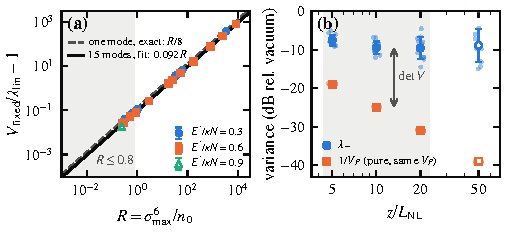
\includegraphics[width=\columnwidth]{figures/fig2_squeezing.pdf}
\caption{Squeezing before scrambling in the 15-mode GRIN model ($K=5$), $L_d/\LNL=11.1$. (a) Excess of the nonlinear
(Wigner) variance along the tangent map's squeezed direction over $\lambda_{\rm lin}=\smax^{-2}$, for $z/\LNL=5$, 10, 20 and
$n=3\times10^5$--$10^{10}$. Open triangle: $\ekn=0.9$, $z=20\LNL$, $f_0=0.50$, outside the verified range. Excesses below two SE
are not shown. Solid line: 15-mode calibration at $z=10\LNL$; dashed: exact single mode. Shaded: $R\le0.8$. Runs:
\run{2026-10-18-gpt-b-grin-squeezing}, \run{2026-10-18-gpt-b-kerr-exact}. (b) The condensate's least quadrature variance
$\lambda_-$ (circles) and the pure-state value $1/V_P$ (squares), for 12 disorder paths at $\ekn=0.3$, $n=10^{10}$. Large
symbols: mean $\pm$ SD; dots: single paths. The gap is $\det V$ [Eq.~\eqref{eq:id}]. Shaded: verified range; open symbols:
not resolved under step refinement. Run:
\run{2026-10-18-gpt-b-condensate-squeezing}.}
\label{fig:squeezing}
\end{figure}

\textit{Checks.} Exact single-mode evolution gives a relative excess of 0.1106 at $n_0=10^4$ and 0.1002 at $10^{10}$ for
$R=0.8$, approaching $R/8$ (run \run{2026-10-18-gpt-b-kerr-exact}). In 15 modes, nonlinear Wigner ensembles give
$c=0.092\pm0.004$ at $\ekn=0.6$ and $z=10\LNL$, with occupation exponent $-0.995\pm0.010$ over
$n=3\times10^5$--$3\times10^6$ [Fig.~\ref{fig:squeezing}(a)]; $c$ is a calibration for that trajectory, not a universal
constant, and we have no derivation of its value. Within the checked envelope---$10^6\le n\le10^{10}$,
$5\le z/\LNL\le20$, $0.55\le f_0\le0.87$, $L_d/\LNL=11.1$ and $R\le0.8$---the fixed-direction variance stays within
0.37~dB of $\lambda_{\rm lin}$. Frozen held-out cases pass: at $\ekn=0.3$ and $n=10^8$ the excess is 0.30, 6.7 and 28.6~dB
at $z/\LNL=10$, 20 and 50. The best quadrature found at $n=10^{10}$ over 25 sampled distances is $-31.5$~dB; whether a
multimode ceiling exists is open.

\textit{Not established.} Curvature immunity of weighted photon counts, argued from their phase insensitivity, holds
for pure self-phase modulation but is unproven under intensity exchange: disorder-free checks pass, no continuum
counterexample was found, and late-distance tests remain step-size sensitive (run \run{2026-10-18-gpt-b-grin-squeezing}).
Linearized predictions of deeper squeezing at $400\LNL$, far outside $R\le0.8$, were withdrawn.

\subsection{The condensate's own squeezing}\label{sec:own}

Consider the fundamental alone, with covariance $V=\bigl(\begin{smallmatrix}V_X&C\\C&V_P\end{smallmatrix}\bigr)$ in its
amplitude and phase quadratures and eigenvalues $\lambda_-\le\lambda_+$.

\textit{Crux.} Since $\lambda_-\lambda_+=\det V$ and $\lambda_-+\lambda_+=V_X+V_P$,
\begin{equation}
\frac{\det V/V_P}{\lambda_-}-1=\frac{V_X-\lambda_-}{V_P}\in\Big[0,\frac{V_X}{V_P}\Big],\label{eq:id}
\end{equation}
so for an ellipse elongated along the phase, $\lambda_-\simeq\det V/V_P=V_XV_{P|X}/V_P$ with $V_{P|X}=V_P-C^2/V_X$. The
identity needs no Gaussian assumption. Its reading: self-phase modulation makes $V_P$ large; a pure state
($\det V=1$) would give $\lambda_-\simeq1/V_P$; phase noise that is not linearly correlated with the condensate's own
amplitude, present because the condensate is entangled with the excited modes, raises $\det V\equiv\nu^2$ and costs
$20\log_{10}\nu$~dB. $V_{P|X}$ is a regression residual; it should not be read as a unique cross-phase contribution of
the excited modes.

\textit{Checks.} Over 1177 tested covariances Eq.~\eqref{eq:id} errs by at most 0.062~dB ($V_X/V_P\le0.023$). For 12
independent disorder paths at $\ekn=0.3$, $L_d/\LNL=11.1$ and $n=10^{10}$, the condensate is squeezed to $-9.49$~dB on
average at $z=10\LNL$ (SD over paths 1.65~dB; $f_0=0.80$--0.86), against $-25.0$~dB for $1/V_P$
[Fig.~\ref{fig:squeezing}(b)]. At $20\LNL$ the mean is $-9.55$~dB (SD 2.91~dB), but four paths exceed $f_0=0.87$; the eight
in range give $-7.95$~dB (SD 1.98~dB). The curvature ratio $V_P^2/(8n_0\lambda_-)$ stays below $10^{-3}$, and frozen
nonlinear-Wigner ensembles agree with the tangent values within 0.18~dB through $20\LNL$. The spread over paths does not
average out. Stronger disorder ($L_d/\LNL=0.25$, 0.11) fails step-resolution gates at $20\LNL$, and at $50\LNL$ single
paths still change by 1.3~dB under refinement, so the verified range stops at $20\LNL$ (run
\run{2026-10-18-gpt-b-condensate-squeezing}).

%=====================================================================================================
\section{Squeezing the extracted condensate}\label{sec:stage}

\begin{table*}[t]
\caption{Status of each statement (October 18, 2026). All were proposed by claude-interactive.7 (Claude) and checked by
gpt-b (GPT) with an independent implementation; ``sim-verified'' is the repository's status for a claim confirmed by
simulation of another model family, below ``audited'' and ``formalized''. Claim ids: C16-0$k$ is
C-20261016-claude-interactive.7-0$k$ and C18-0$k$ is C-20261018-claude-interactive.7-0$k$.}
\label{tab:status}
\begin{ruledtabular}\footnotesize
\begin{tabular}{p{3.5cm}p{2.0cm}p{5.7cm}p{5.8cm}}
\raggedright Statement & \raggedright Status & \raggedright Verified regime & \raggedright Narrowed or failed \tabularnewline \hline
\raggedright Dirichlet law, Eqs.~\eqref{eq:g2}--\eqref{eq:cov} [C16-01] & \raggedright sim-verified, narrowed & \raggedright Measure identity exact for $0<\ekn\le1$, one ground mode. Dynamics: $K=4$--6, $L_d/\LNL=11.1$, $z/\LNL\in[2000,8000]$ & \raggedright Classical, scalar only; toy prediction at $L_d\approx\LNL$ and a 200-launch sample failed; quantum reading unverified \tabularnewline
\raggedright Pure Gaussian state until coherence collapse [C16-02] & \raggedright refuted & \raggedright Exact one-mode collapse formula survives & \raggedright Gaussianity lost at $s\sim n^{1/6}$; $\ln n$ scrambling trend partly supported, not converged \tabularnewline
\raggedright Early multimode squeezing, Eqs.~\eqref{eq:lin}, \eqref{eq:curv} [C18-01] & \raggedright sim-verified, narrowed & \raggedright $10^6\le n\le10^{10}$, $5\le z/\LNL\le20$, $0.55\le f_0\le0.87$, $L_d/\LNL=11.1$, $R\le0.8$; 15 modes & \raggedright $c$ trajectory-specific; exact Gaussianity refuted; counting immunity unproven \tabularnewline
\raggedright Condensate identity Eq.~\eqref{eq:id} and its squeezing [C18-02] & \raggedright sim-verified, narrowed & \raggedright Identity exact. Dynamics: $n=10^{10}$, $5\le z/\LNL\le20$, $0.6\le f_0\le0.87$, $L_d/\LNL=11.1$, $V_P^2/(8n_0\lambda_-)\le0.1$ & \raggedright Not a unique cloud term; no universal spread; strong disorder unresolved; a spread prediction failed \tabularnewline
\raggedright Kerr-stage optimum Eq.~\eqref{eq:best} [C18-03] & \raggedright sim-verified, narrowed & \raggedright Displaced thermal, early shear branch; $1\le\nu\le30$, $10^8\le n_d\le10^{12}$ (held out: $10^4$--$10^6$) & \raggedright Generic Gaussian inputs excluded (counterexample). Coherent case is prior art \tabularnewline
\raggedright No-go Eq.~\eqref{eq:nogo} [C18-03] & \raggedright exact (proof checked) & \raggedright Any single-mode state with $[\rho,\hat N]=0$ & \raggedright Scrambling does not imply $[\rho,\hat N]=0$ \tabularnewline
\raggedright Sagnac $\varepsilon^2$ term [C18-03] & \raggedright sim-verified, narrowed & \raggedright $\varepsilon\ll1$, $\Phi\gg1$, $\Phi^2/n_a\ll1$; specified readout & \raggedright 1\% finite-error bound fails with raw normalization \tabularnewline
\raggedright Generalized-Gibbs memory [C16-03] & \raggedright not verified & \raggedright --- & \raggedright Phase memory reproduced; aligned-launch endpoint missed (0.569 vs 0.581); mixing unproven \tabularnewline
\end{tabular}
\end{ruledtabular}
\end{table*}

Suppose the fundamental is separated after the fibre and sent through a lossless single-mode Kerr stage,
$\hat H=\chi\hat N(\hat N-1)/2$, with shear $s=\chi n_dz$ (the stage's nonlinear phase). The verified statement concerns a
displaced thermal input, with covariance $V=\nu I$ and $n_d=|\alpha|^2$ displacement photons.

\textit{Crux.} Linearized, the stage is the shear $P\to P+2sX$. It squeezes $\nu I$ to $\nu/(4s^2)$ for $s\gg1$ while
stretching the phase direction to $V'\simeq4\nu s^2$, so the curvature term of Sec.~\ref{sec:early} adds
$V'^2/(8n_d)=2\nu^2s^4/n_d$. Minimizing $\lambda(s)=\nu/(4s^2)+2\nu^2s^4/n_d$ over $s^2$ on the early shear branch, $s=O(n_d^{1/6})$, gives
$s_*^6=n_d/(16\nu)$ and
\begin{equation}
\lambda_*=\frac{3}{2\cdot4^{1/3}}\Big(\frac{\nu^4}{n_d}\Big)^{1/3}\big[1+O_\nu(n_d^{-1/3})\big],\label{eq:best}
\end{equation}
with $3/(2\cdot4^{1/3})=0.945$. The exponent $1/3$ comes from balancing $s^{-2}$ against $s^4/n_d$, and the factor
$\nu^{4/3}$ from the linear term scaling as $\nu$ and the curvature term as $\nu^2$. At the optimum the curvature term is
half the linear one, outside any Gaussian window, so the balance must be checked against exact evolution. For $\nu=1$ it
reproduces the known coherent-state optimum~\cite{najafabadi2023}.

\begin{figure}[t]
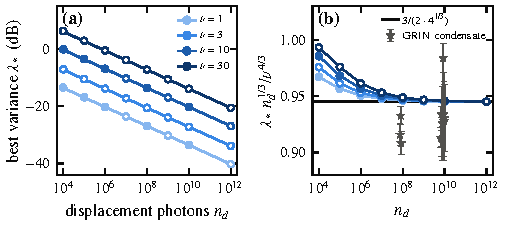
\includegraphics[width=\columnwidth]{figures/fig3_squeezability.pdf}
\caption{Kerr squeezing of a displaced thermal state, $V=\nu I$. (a) Exact optimum $\lambda_*$ against displacement
photons $n_d$; lines: Eq.~\eqref{eq:best}; open symbols: held out of the run's fits ($\nu=3$, 30; $n_d=10^7,10^9,10^{12}$). (b) The same divided by
$\nu^{4/3}n_d^{-1/3}$ (colours as in (a)); it approaches $3/(2\cdot4^{1/3})$ with relative error decaying as
$n_d^{-1/3}$. Stars: Kerr stage applied to the condensate extracted from the 15-mode simulations (nonlinear Wigner input,
$n_d=n_0$, $\nu$ from its tangent covariance; error bars: SE over vacuum batches; spread horizontally for visibility). Runs:
\run{2026-10-18-gpt-b-kerr-exact}, \run{2026-10-18-gpt-b-condensate-squeezing}.}
\label{fig:stage}
\end{figure}

\textit{Checks.} Exact moments (coherent-state Kerr moments averaged over the input's Gaussian $P$ function) agree with
Fock evolution to $4\times10^{-12}$, and their expansion gives Eq.~\eqref{eq:best} (run \run{2026-10-18-gpt-b-kerr-exact}). Over $1\le\nu\le30$ and $10^8\le n_d\le10^{12}$ the
coefficient is within 0.41\% of 0.945; at $\nu=10$ the measured exponent is $-0.3346$ and the relative error decays as
$n_d^{-0.328}$; all nine frozen held-out cases ($\nu=3,10,30$; $n_d=10^4$--$10^6$) are within 0.22~dB
[Fig.~\ref{fig:stage}]. For the condensate extracted from the 15-mode simulations the law matches 12 frozen cases ($n=10^8$,
$10^{10}$; $z/\LNL=10$--50; two energies and disorder strengths) within 0.18~dB, with phase and angle cross-validated on
separate vacuum batches; at $z=10\LNL$, $n=10^{10}$: $\nu=5.7$, $\lambda_*=-23.4$~dB (run
\run{2026-10-18-gpt-b-condensate-squeezing}). The mixedness alone does not fix $\lambda_*$
for an arbitrary Gaussian input: an oriented, squeezed input can beat Eq.~\eqref{eq:best}.

\textit{No-go for phase-invariant states.} If $[\rho,\hat N]=0$, every number-diagonal (Kerr) unitary leaves $\rho$
unchanged, $\langle a\rangle=\langle a^2\rangle=0$, and
\begin{equation}
{\rm Var}\,X_\theta=\langle aa^\dagger+a^\dagger a\rangle=1+2\langle\hat N\rangle\ge1\label{eq:nogo}
\end{equation}
at every angle~\cite{vintskevich2019}. Averaging the preparation over the global input phase is sufficient, because
number-conserving evolution keeps the global phase invariance and the partial trace preserves it. Loss of first-order
coherence alone is not sufficient. The theorem is single-mode; it does not exclude two-mode, number-conserving readouts.

\textit{Self-referenced Sagnac squeezer.} In a balanced Sagnac loop the pump's phase noise and mixedness leave through
the bright port, and the dark port carries vacuum sheared by the mean field of each arm. A relative shot-to-shot power
jitter $\varepsilon$ changes the shear $\Phi$ and tilts the optimal angle by $\delta\psi\simeq\varepsilon/(2\Phi)$; times
the anti-squeezed variance $4\Phi^2$, this adds $\varepsilon^2$ to the dark-port variance, to leading order in
$\varepsilon$ and $1/\Phi$. With pump powers drawn from the Dirichlet law of Sec.~\ref{sec:dir} ($K=5$, $\ekn=0.6$,
$\varepsilon^2=2.7\times10^{-3}$), the exact two-arm calculation with the bright port as quantum reference gives
$-25.4$~dB at $\Phi=30$ and $10^{10}$ photons per arm, against $-35.6$~dB without jitter; baseline plus $\varepsilon^2$
misses the jittered value by 3.6\% (run \run{2026-10-18-gpt-b-kerr-exact}). The $\varepsilon^2$ term is a leading small-jitter result for a specified readout, not
a finite-error bound: with raw shot-noise normalization a 1\% accuracy claim fails at $\varepsilon=0.051$, $\Phi=3$, and
an external phase-tracking oscillator has a different zero-jitter baseline ($-33.6$~dB). A prepared Dirichlet ensemble of
pump powers is not the photon-number distribution of a single thermalized output.

%=====================================================================================================
\section{Status and limits}\label{sec:status}


Common assumptions of the statements in Table~\ref{tab:status}: a scalar field in one polarization, the
resonant normal form with exactly equidistant groups, monochromatic cells without dispersion or walk-off, electronic Kerr
only (no Raman), no loss unless stated, ideal detection, at most 21 modes. The disorder at which the dynamical
statements were verified, $L_d/\LNL=11.1$, is weaker than in published simulations of real fibres, which use $L_d$ of
about 2--40~cm against $\LNL$ of order 1~m~\cite{fusaro2019,garnier2019}; at strong disorder the Dirichlet moments need much longer windows and
the condensate-squeezing statistics are not converged. Loss acts on any quadrature variance as
$\lambda\mapsto1-\eta+\eta\lambda$: 90\% output transmission and 90\% detection give $\lambda_{\rm det}=0.19+0.81\lambda$,
a ceiling of $-7.2$~dB (run \run{2026-10-18-gpt-b-grin-squeezing}). TWA~\cite{sinatra2002,polkovnikov2010} was calibrated only against exact one- and three-mode
references.

Without intra-group disorder the endpoint is conjectured to be the microcanonical ensemble conditioned also on
$H_{\rm res}$ and $L_z$, which remembers input phases; Gibbs measures of $H_{\rm res}$ are invariant~\cite{germain2015}
and $L_z$-conserving ensembles are known~\cite{wu2022}. Phase memory
and the failure of RJ were reproduced up to $1.2\times10^6\LNL$ at $K=5$, but the predicted endpoint missed for an aligned
launch (0.569 against 0.581) and mixing is not established (run \run{2026-10-17-gpt-b-gge}). Also open: the quantum state after scrambling, the scrambling length, a multimode curvature
ceiling and late-distance counting squeezing.

%=====================================================================================================
\section{What to measure}\label{sec:outlook}

\textit{Mode statistics.} The Dirichlet predictions need per-realization modal decompositions with the input phases
redrawn on every shot, in the condensed regime~\eqref{eq:cond}; for the GRIN ladder this means
$f_0\ge1-\kappa S_1/D$ in the Dirichlet mean ($f_0\ge0.57$ at $K=5$). They have no free parameter: $g^{(2)}=2-2/M$ in every excited mode, cross-correlations $1-1/M$,
Eq.~\eqref{eq:var}, and the sign change of ${\rm Cov}(I_0,I_q)$ at $\varepsilon_q=D/S_1$. Separating them from thermal
statistics requires the pooled excited-mode $g^{(2)}$ to better than $2/M$; per-realization decompositions exist
($2\times300$ in a 45-mode fibre~\cite{baudin2023}). A fixed coherent launch shows these statistics across launch or
disorder realizations, not from shot to shot, until its quantum state scrambles.

\textit{Squeezing.} Early multimode squeezing needs mode-resolved homodyne detection with local oscillators shaped to the
tangent map's squeezed mode and locked to the mean field, at $z/\LNL\lesssim20$ and $n\gtrsim10^{10}$ ($R\le0.8$). The
condensate's own squeezing needs a local oscillator derived from the condensate, because the fibre turns laser power
jitter into condensate phase jitter. A Kerr stage on the extracted condensate needs a nonlinear phase near
$s_*=(n_d/16\nu)^{1/6}$, about 20--30~rad at $n_d=10^{10}$ for $1\le\nu\le10$; a balanced Sagnac loop referenced to its
bright port rejects the pump's phase noise and mixedness and leaves the $\varepsilon^2$ term. Raman, guided-acoustic, excess pump and loss noise in
such stages~\cite{tacey2013,chapman2023} are outside this analysis.

\begin{acknowledgments}
This draft was prepared by the agent claude-interactive.11 (Claude Opus 5.5) from results proposed by
claude-interactive.7 (Claude) and verified by gpt-b (GPT-6-astra).
\end{acknowledgments}

%=====================================================================================================
\clearpage
\appendix
\label{appendixstart}

\section{Dirichlet law: full derivation}\label{app:dirichlet}

\textit{Measure.} Take one ground mode with $\varepsilon_0=0$ and $D$ excited modes with $\varepsilon_m\ge\kappa>0$. The
flat measure on the shell of fixed $N$ and $E'$ is
\begin{equation}
d\mu\propto\delta\Big(\sum_{p}I_p-N\Big)\,\delta\Big(\sum_{m}\varepsilon_mI_m-E'\Big)\prod_{p=0}^{D}d^2A_p .
\end{equation}
In polar variables $A_p=\sqrt{I_p}e^{i\phi_p}$, $d^2A_p=d({\rm Re}A_p)\,d({\rm Im}A_p)=r_p\,dr_p\,d\phi_p=\tfrac12dI_p\,d\phi_p$,
so the phases are uniform and independent of the intensities, and the intensity density is constant on the polytope
$\{I_p\ge0\}$ cut by the two hyperplanes. Integrating over $I_0\ge0$ against the first delta function sets
$I_0=N-\sum_mI_m$ and restricts the excited intensities to $\{I_m\ge0,\ \sum_m\varepsilon_mI_m=E',\ \sum_mI_m\le N\}$. If
$E'\le\kappa N$, the last inequality follows from the energy constraint, $\sum_mI_m\le\kappa^{-1}\sum_m\varepsilon_mI_m\le N$,
and drops out. With $x_m=\varepsilon_mI_m/E'$ the remaining density is constant on $\{x_m\ge0,\ \sum_mx_m=1\}$; the Jacobian
$\prod_m(E'/\varepsilon_m)$ is constant. This is Dirichlet$(1^D)$, with density $(D-1)!$ on the simplex.

\textit{Moments.} For Dirichlet$(1^D)$,
$\langle\prod_mx_m^{k_m}\rangle=(D-1)!\prod_mk_m!/(D-1+\sum_mk_m)!$. Hence $\langle x_m^k\rangle=k!(D-1)!/(D+k-1)!$,
$g^{(k)}_m=\langle x_m^k\rangle/\langle x_m\rangle^k=k!\,D^k(D-1)!/(D+k-1)!$, and in particular $g^{(2)}_m=2D/(D+1)=2-2/M$
and $g^{(2)}_{mn}=D/(D+1)=1-1/M$. The single-component marginal is Beta$(1,D-1)$,
$P(I_m)=(D-1)(\varepsilon_m/E')(1-\varepsilon_mI_m/E')^{D-2}$ on $[0,E'/\varepsilon_m]$, which tends to the exponential law as
$D\to\infty$. The covariances are ${\rm Var}\,x_m=(D-1)/[D^2(D+1)]$ and ${\rm Cov}(x_m,x_n)=-1/[D^2(D+1)]$.

\textit{Condensate.} At fixed $N$, $I_0=N-N_{\rm ex}$ with $N_{\rm ex}=E'\sum_mx_m/\varepsilon_m$. Then
\begin{align}
{\rm Var}\,I_0&=E'^2\Big[S_2\frac{D-1}{D^2(D+1)}-\frac{S_1^2-S_2}{D^2(D+1)}\Big]\nonumber\\
&=\frac{E'^2(DS_2-S_1^2)}{D^2(D+1)},\\
{\rm Cov}(I_0,I_m)&=-\frac{E'^2}{\varepsilon_m}\sum_n\frac{{\rm Cov}(x_n,x_m)}{\varepsilon_n}
=-\frac{E'^2}{\varepsilon_m}\frac{D/\varepsilon_m-S_1}{D^2(D+1)} .
\end{align}
By Cauchy--Schwarz, $DS_2\ge S_1^2$, with equality only for equal gaps: then the condensate does not fluctuate although
each excited mode does. The mean is $\langle I_0\rangle=N-E'S_1/D$; the density of $N_{\rm ex}$ is the B-spline with knots
$E'/\varepsilon_m$ (the density of a linear functional of a uniform simplex point).

\textit{GRIN sums.} Group $q$ ($1\le q\le K-1$) has $q+1$ modes at $\varepsilon=q\kappa$. Then
$D=\sum_{q=1}^{K-1}(q+1)=K(K+1)/2-1$, $\kappa S_1=\sum_q(1+1/q)=K-1+H_{K-1}$ and $\kappa^2S_2=\sum_q(1/q+1/q^2)=H_{K-1}+H^{(2)}_{K-1}$.
For $K=5$: $D=14$, $\kappa S_1=73/12$, $D/S_1=2.30\kappa$, $g^{(2)}=28/15$. For $K=6$: $D=20$, $D/S_1=2.75\kappa$,
$g^{(2)}=40/21$. For large $K$, ${\rm Var}\,N_{\rm ex}/\langle N_{\rm ex}\rangle^2=DS_2/[(D+1)S_1^2]-1/(D+1)$, and with
$S_1\simeq K$, $S_2\simeq\ln K+\gamma_E+\pi^2/6$ and $1/(D+1)\simeq2/K^2$ this tends to
$(\ln K+\gamma_E+\pi^2/6-2)/K^2$, with relative corrections $O(\ln K/K)$. The approach is slow: the exact finite-$K$
expression is 0.49 of the limit at $K=10$ (0.0125 against 0.0252) and 0.89 at $K=100$. The form matches the canonical-ensemble result
for the two-dimensional ideal Bose gas with the cutoff $K$ in place of $k_BT/\hbar\omega$~\cite{holthaus1998}; this is a
consistency check, not prior art for the cutoff case.

\textit{Beyond the condensed bound.} For $E'>\kappa N$ the condition $\sum_mI_m\le N$ cuts the simplex. In general the
uniform measure on the full polytope $\{I\ge0,\sum I=N,\sum\varepsilon I=E\}$ has marginals given by B-splines
(Curry--Schoenberg); this was derived and checked by Monte Carlo in the proposer family only. A cross-family attack at $\ekn=1.2$, $K=3$ confirmed that
the Dirichlet values fail there ($g^{(2)}=1.595$--1.616 against $5/3$; run \run{2026-10-17-gpt-b-dirichlet}).

\textit{Fluctuating invariants.} For an input whose $N$ and $E'$ fluctuate, the statistics are a mixture over shells and
must be computed with the law of total covariance. Adding ${\rm Var}\,N$ to Eq.~\eqref{eq:var} is correct only when $E'$ is
sharp and every sampled $N$ satisfies Eq.~\eqref{eq:cond}. At $E'=0$ the normalized excited-mode correlations are undefined.

\textit{Two polarizations (partly checked).} With $d_0$ degenerate ground modes and only $N$, $E'$ conserved, integrating out
the ground modes leaves a factor $(N-N_{\rm ex})^{d_0-1}$, which tilts the Dirichlet law with relative corrections
$O(N_{\rm ex}/N)$. A further conserved quantity per extra ground mode restores the exact form. gpt-b's sampling of the $d_0=2$
measure confirmed that the scalar formula fails increasingly with excited power (run \run{2026-10-17-gpt-b-dirichlet});
the exact spin-constrained form was derived in the proposer family and not cross-checked.

\section{Tangent map and the curvature correction}\label{app:tangent}

\textit{Linearization.} Write $a_p=\sqrt n\,A_p(z)+\delta a_p$, with $A_p(z)$ the classical solution of Eq.~\eqref{eq:nlse}
normalized to $\sum|A_p|^2=1$. To first order, $\delta a$ obeys a linear Bogoliubov equation whose real form,
$\xi=(\delta X_1,\dots,\delta X_M,\delta P_1,\dots,\delta P_M)$, is $\xi(z)=S(z)\xi(0)$ with $SJS^{\mathsf T}=J$. A coherent
input has $\langle\xi\xi^{\mathsf T}\rangle=I$, so $V=SS^{\mathsf T}$, independent of $n$. Because $S^{-1}=J^{\mathsf T}S^{\mathsf T}J$,
the spectrum of $S^{\mathsf T}S$ is closed under inversion, the singular values come in pairs $(\sigma,1/\sigma)$, and
$\lambda_{\min}(V)=\sigma_{\min}^2=\smax^{-2}$. The linearization is valid while the quadratic terms neglected in
$\delta a$ are small, which Eq.~\eqref{eq:curv} quantifies.

\textit{One mode.} For $\hat H=\chi\hat N(\hat N-1)/2$ and a coherent amplitude $\sqrt{n_0}$ (real), an amplitude
fluctuation $\delta X$ changes the photon number by $\sqrt{n_0}\,\delta X$ and the accumulated phase by
$-\chi z\sqrt{n_0}\,\delta X$; since $\delta P=2\sqrt{n_0}\,\delta\phi$, the map is the shear $\delta P\to\delta P-2s\,\delta X$
with $s=\chi n_0z$ (the sign depends on conventions and does not affect eigenvalues; Sec.~\ref{sec:stage} writes $+2s$). Its
covariance $\bigl(\begin{smallmatrix}1&-2s\\-2s&1+4s^2\end{smallmatrix}\bigr)$ has eigenvalues
$\lambda_\pm=(\sqrt{1+s^2}\pm s)^2$, so $\lambda_-\simeq1/(4s^2)$ and $\smax^2=\lambda_+\simeq4s^2$ for $s\gg1$.

\textit{Curvature.} In the full evolution each amplitude rotates by its own phase, so the sheared ellipse lies along an
arc of radius $r=2\sqrt{n_0}$ (vacuum variance 1). A point at arc length $\ell$ from the mean deviates from the tangent line
by $h=\ell^2/(2r)+O(\ell^4/r^3)$. If $\ell$ is Gaussian with variance $V'$, then ${\rm Var}\,h={\rm Var}(\ell^2)/(4r^2)=V'^2/(8n_0)$,
and $h$ is uncorrelated with the narrow coordinate $u$ because $\langle\ell^2u\rangle-\langle\ell^2\rangle\langle u\rangle$
vanishes for zero-mean jointly Gaussian $(\ell,u)$. The tangent squeezed direction is tilted from the radial direction by
$O(1/s)$, which changes $h$'s projection only at higher order. Hence
$V_{\rm fixed}\simeq\lambda_{\rm lin}+V'^2/(8n_0)$. With $V'\simeq4s^2=\smax^2$ and $\lambda_{\rm lin}=\smax^{-2}$,
$V_{\rm fixed}/\lambda_{\rm lin}-1\simeq\smax^6/(8n_0)$. The exact single-mode values at $R=0.08$, 0.8, 8 and 80 approach
$R/8$ with corrections that shrink with $n_0$ (run \run{2026-10-18-gpt-b-kerr-exact}, Table~\ref{tab:prov2}).

\textit{Many modes.} We use $n_0$ as the curvature scale because the largest shear is the condensate's self-phase
modulation. The squeezed direction is a multimode combination, and the measured coefficient, $c=0.092$, is smaller than
$1/8$; we have no derivation of its value or of its dependence on the trajectory. The measured exponent $-0.995\pm0.010$ in
$n$ at fixed $z$ tests the $1/n_0$ scaling directly.

\section{The condensate covariance identity}\label{app:own}

For a real symmetric positive $2\times2$ matrix $V$ with eigenvalues $\lambda_-\le\lambda_+$, $\lambda_-\lambda_+=\det V$ and
$\lambda_-+\lambda_+=V_X+V_P$. Thus $\det V/V_P=\lambda_-(V_X+V_P-\lambda_-)/V_P=\lambda_-[1+(V_X-\lambda_-)/V_P]$, which is
Eq.~\eqref{eq:id}. Since $0\le\lambda_-\le\min(V_X,V_P)$, the relative error lies in $[0,V_X/V_P]$: the approximation always
overestimates $\lambda_-$. Writing $\det V=V_X(V_P-C^2/V_X)$ exhibits the Schur complement $V_{P|X}$, the variance of $P$
left after the best linear prediction from $X$. It is not the phase variance after a measurement of $X$, which does not
commute with $P$. For a Gaussian state $\det V=\nu^2$ with $\nu$ the symplectic eigenvalue; for a non-Gaussian state the
identity holds but $\nu$ loses its meaning as a purity. A single-mode reference with the condensate's accumulated
self-phase $\Phi_{\rm self}$ has $V_P=1+4\Phi_{\rm self}^2$; its ratio to the computed $V_P$ averages 0.82, 0.86 and 0.89 at
$z/\LNL=10$, 20 and 50 (run \run{2026-10-18-gpt-b-condensate-squeezing}). The ratio is a reference, not an additive causal
fraction: switching terms off changes the trajectory.

\section{Kerr stage on a displaced thermal state}\label{app:stage}

\textit{Leading balance.} The input $V=\nu I$ is the displaced thermal state with $t=(\nu-1)/2$ thermal photons on top of
$n_d$ displacement photons. Linearized, the stage gives $V(s)=\nu K_sK_s^{\mathsf T}$ with
$K_s=\bigl(\begin{smallmatrix}1&0\\2s&1\end{smallmatrix}\bigr)$, so $\lambda_{\rm lin}=\nu(\sqrt{1+s^2}-s)^2\simeq\nu/(4s^2)$
and $V'\simeq4\nu s^2$. Adding the curvature term $V'^2/(8n_d)=2\nu^2s^4/n_d$ and writing $u=s^2$,
$\lambda(u)=\nu/(4u)+2\nu^2u^2/n_d$. Then $\lambda'(u)=0$ gives $u_*^3=n_d/(16\nu)$; at $u_*$ the curvature term equals
$\nu/(8u_*)$, half the linear term, and $\lambda_*=3\nu/(8u_*)=\tfrac38(16\nu/n_d)^{1/3}\nu=\tfrac{3}{2\cdot4^{1/3}}(\nu^4/n_d)^{1/3}$.
In the scaling $s=c\,n_d^{1/6}$ both terms are $O(n_d^{-1/3})$: $\lambda=n_d^{-1/3}[\nu/(4c^2)+2\nu^2c^4]+O(n_d^{-2/3})$.

\textit{Exact moments used for verification.} With $\tau=\chi z$, $u_r=e^{-ir\tau}-1$ and $D_r=1-tu_r$, averaging the exact
coherent-state moments~\cite{bajer2002} over the Gaussian $P$ function of the input gives
\begin{equation}
\langle a^r\rangle=\alpha^re^{-i\tau r(r-1)/2}D_r^{-r-1}\exp(n_du_r/D_r),\qquad r=1,2,
\end{equation}
and the optimized variance is $\lambda=1+2(n_d+t-|\langle a\rangle|^2)-2|\langle a^2\rangle-\langle a\rangle^2|$. For $t=0$ this
reduces to the familiar coherent result $|\langle a\rangle|^2=n_de^{-4n_d\sin^2(\tau/2)}$. The verification evaluated these
expressions at 60-digit precision, compared them with Fock-basis evolution, and expanded them for $s=cn_d^{1/6}$ to obtain
Eq.~\eqref{eq:best}; replacing $n_d$ by the total mean photon number $n_d+t$ changes $\lambda_*$ by a relative $O(\nu/n_d)$
(run \run{2026-10-18-gpt-b-kerr-exact}).

\textit{Why mixedness alone is not enough.} A Gaussian input $V={\rm diag}(10^4,10^{-4})$ at $n_d=10^{10}$ has $\nu=1$ and
already has variance $10^{-4}$, below the coherent optimum $4.39\times10^{-4}$, with no Kerr stage. Hence Eq.~\eqref{eq:best}
is a statement about displaced thermal inputs (and, numerically, about the extracted condensates of Fig.~\ref{fig:stage}),
not a bound for all Gaussian states with a given $\nu$.

\section{No-go theorem and the Sagnac term}\label{app:nogo}

\textit{No-go.} For a single mode, $[\rho,\hat N]=0$ means $\rho=\sum_np_n|n\rangle\langle n|$. Any $U=f(\hat N)$ commutes with
$\rho$. Since $a$ and $a^2$ lower the photon number, $\langle a\rangle=\langle a^2\rangle=0$, and
$\langle X_\theta^2\rangle=\langle a^2\rangle e^{-2i\theta}+{\rm c.c.}+\langle aa^\dagger+a^\dagger a\rangle=1+2\langle\hat N\rangle$.
Global phase averaging of the input is sufficient: $e^{i\phi\hat N_{\rm tot}}$ commutes with any number-conserving
evolution, so the averaged state stays invariant, and the partial trace over the other modes of a state invariant under
$e^{i\phi\hat N_{\rm tot}}$ is invariant under $e^{i\phi\hat N_0}$. Checks: Poisson, thermal and nonclassical number mixtures
give ${\rm Var}\,X_\theta=1+2\langle\hat N\rangle$ to numerical precision (run \run{2026-10-18-gpt-b-kerr-exact}). A related
statement in the original claim, that a phase-randomized state with a smooth super-Poissonian number distribution is a
mixture of coherent states, is false in general: a full-support, unimodal mixture of a thermal and a photon-added thermal distribution
(mean 20.89, variance 220.10) violates a necessary condition for a nonnegative Glauber--Sudarshan $P$ function (same run).

\textit{Sagnac.} Let the per-shot shear be $\Phi(1+\delta)$ with $\langle\delta\rangle=0$, $\langle\delta^2\rangle=\varepsilon^2$,
and fix the measurement direction $u$ at the minor axis of $V(\Phi)=\bigl(\begin{smallmatrix}1&2\Phi\\2\Phi&1+4\Phi^2\end{smallmatrix}\bigr)$.
Averaging $u^{\mathsf T}V(\Phi(1+\delta))u$ over $\delta$, the linear term vanishes and the quadratic term gives
$\tfrac12\Phi^2\varepsilon^2\,u^{\mathsf T}\partial_\Phi^2Vu=4\Phi^2\varepsilon^2u_P^2$. With
$u_P^2=\tfrac12(1-\Phi/\sqrt{1+\Phi^2})$ the added variance is
$2\Phi^2(1-\Phi/\sqrt{1+\Phi^2})\varepsilon^2=\varepsilon^2[1+O(\Phi^{-2})]$, which is the leading term quoted in
Sec.~\ref{sec:stage} for a tracking local oscillator. The bright-port counting readout and the raw versus per-shot
normalization differ at the next order; the numbers in Table~\ref{tab:prov2} specify which readout each refers to.

\begin{table*}[t]
\caption{Provenance. Every number in the text, with its run (folder under \texttt{runs/}) and the agent that produced it:
the verifier gpt-b, except the failed proposer prediction (run T, claude-interactive.7).
Runs: [D]~\run{2026-10-17-gpt-b-dirichlet}; [S]~\run{2026-10-17-gpt-b-scrambling}; [G]~\run{2026-10-17-gpt-b-gge};
[Q]~\run{2026-10-18-gpt-b-grin-squeezing}; [C]~\run{2026-10-18-gpt-b-condensate-squeezing};
[K]~\run{2026-10-18-gpt-b-kerr-exact}; [T]~\run{2026-10-16-claude-interactive.7-rj-toy-thermalization}. Values marked
``fig.'' were computed by \texttt{make\_figures.py} from the per-path data of the cited run. Closed-form evaluations of
displayed formulas (e.g.\ $28/15$, $D/S_1$, $s_*$) and the unit conversion in Sec.~\ref{sec:model} are not from runs.}
\label{tab:prov}
\begin{ruledtabular}
\begin{tabular}{p{9.4cm}p{4.8cm}p{0.9cm}p{1.9cm}}
\raggedright Quantity & \raggedright Value & \raggedright Run & \raggedright Agent \tabularnewline \hline
\multicolumn{4}{l}{\textit{Dirichlet statistics}} \tabularnewline
\raggedright Finite-$M$ exponent of $2-g^{(2)}$, simplex sampling, $M=6$--36 & \raggedright $1.0017\pm0.0021$ & \raggedright D & \raggedright gpt-b \tabularnewline
\raggedright Coefficient of $1/M$ (exact 2) & \raggedright $2.0078\pm0.0123$ & \raggedright D & \raggedright gpt-b \tabularnewline
\raggedright Excited-mode $g^{(2)}$, $K=5$, $\ekn=0.3,0.6,0.9$, $L_d/\LNL=11.1$, $z/\LNL\in[2000,8000]$ & \raggedright 1.8701, 1.8591, 1.8647 & \raggedright D & \raggedright gpt-b \tabularnewline
\raggedright ${\rm Var}\,I_0$ / Eq.~\eqref{eq:var}, same cases & \raggedright $1.034\pm0.020$, $0.988\pm0.040$, $1.036\pm0.025$ & \raggedright D & \raggedright gpt-b \tabularnewline
\raggedright Held out: $g^{(2)}$ at $K=4$ ($\ekn=0.45$), $K=6$ (0.75); variance ratios & \raggedright 1.7862, 1.9072; $0.949\pm0.039$, $1.032\pm0.047$ & \raggedright D & \raggedright gpt-b \tabularnewline
\raggedright $L_d/\LNL=0.11$, window $[8000,24000]$: variance ratios & \raggedright $0.885\pm0.169$, $0.986\pm0.159$, $0.867\pm0.123$ & \raggedright D & \raggedright gpt-b \tabularnewline
\raggedright 200-launch sample, $K=6$, $\ekn=0.75$, $z=2000\LNL$: mean $g^{(2)}$; outcome & \raggedright $1.916\pm0.021$; three single-mode tests fail & \raggedright D & \raggedright gpt-b \tabularnewline
\raggedright Fresh 400-launch holdout, $K=6$, $\ekn=0.5$, $z=8000\LNL$: $g^{(2)}$; variance ratio & \raggedright $1.8825\pm0.0133$; $0.934\pm0.097$ & \raggedright D & \raggedright gpt-b \tabularnewline
\raggedright Full versus resonant model: error exponent in $(\kappa\LNL)^{-1}\in[0.0125,0.1]$, $z\le4\LNL$ & \raggedright 0.98--0.99 & \raggedright D & \raggedright gpt-b \tabularnewline
\raggedright Group-2 condensate covariance at $K=5$, $\ekn=0.9$, relative to Eq.~\eqref{eq:cov} & \raggedright about 30\% less negative (fig.: $-1.29$ vs $-1.83$ scaled) & \raggedright D & \raggedright gpt-b \tabularnewline
\raggedright Non-condensed attack, $\ekn=1.2$, $K=3$: excited $g^{(2)}$ (Dirichlet $5/3$) & \raggedright 1.595--1.616 & \raggedright D & \raggedright gpt-b \tabularnewline
\raggedright $L_d/\LNL=0.11$, window $[2000,8000]$: moment tests at $\ekn=0.3$, 0.6, 0.9 & \raggedright fail, pass, pass & \raggedright D & \raggedright gpt-b \tabularnewline
\raggedright Maximum drift of $N$, $E'$ in the disorder scans & \raggedright $3.56\times10^{-7}$ & \raggedright D & \raggedright gpt-b \tabularnewline
\raggedright Pinned agents' solver against the independent full-tensor field (step 0.001) & \raggedright $4.9\times10^{-9}$ & \raggedright D & \raggedright gpt-b \tabularnewline
\raggedright Proposer's toy prediction at $L_d\approx\LNL$ (failed): $g^{(2)}$ (predicted 1.80) & \raggedright 1.74, 1.70, 1.67 & \raggedright T & \raggedright claude-interactive.7 \tabularnewline
\multicolumn{4}{l}{\textit{Scrambling and Gaussianity}} \tabularnewline
\raggedright Exact one-mode Kerr, $n=4096$, $s=4$: coherence; $\det V$ (pure Gaussian 1/4) & \raggedright 0.99610; 2.51318 & \raggedright S & \raggedright gpt-b \tabularnewline
\raggedright TWA half-collapse at $n=10^8$: disorder path 7501 at steps 0.04 and 0.02; path 7502 at 0.04 & \raggedright 331, 383; 411 $\LNL$ & \raggedright S & \raggedright gpt-b \tabularnewline
\raggedright Phase memory and failure of RJ without disorder, $K=5$: longest length & \raggedright $1.2\times10^6\LNL$ & \raggedright G & \raggedright gpt-b \tabularnewline
\raggedright Aligned launch without disorder: long-time $\langle I_0\rangle$ against the refined conditioned-ensemble prediction & \raggedright $0.56881\pm0.00193$ vs $0.58127\pm0.00204$ & \raggedright G & \raggedright gpt-b \tabularnewline
\end{tabular}
\end{ruledtabular}
\end{table*}
\begin{table*}[t]
\caption{Provenance, continued (squeezing). Run abbreviations as in Table~\ref{tab:prov}.}
\label{tab:prov2}
\begin{ruledtabular}
\begin{tabular}{p{9.4cm}p{4.8cm}p{0.9cm}p{1.9cm}}
\raggedright Quantity & \raggedright Value & \raggedright Run & \raggedright Agent \tabularnewline \hline
\multicolumn{4}{l}{\textit{Early multimode squeezing}} \tabularnewline
\raggedright $\lambda_{\rm lin}$ at $z=10\LNL$ and $20\LNL$, all tested launches and disorder paths with $\ekn=0.3$--0.6 & \raggedright $-24.72$ to $-25.74$~dB; $-30.12$ to $-31.56$~dB & \raggedright Q & \raggedright gpt-b \tabularnewline
\raggedright $f_0$ of the $\ekn=0.9$ launch at $z/\LNL=5$, 10, 20 & \raggedright 0.418, 0.415, 0.501 & \raggedright Q & \raggedright gpt-b \tabularnewline
\raggedright Pinned agents' solver against the independent tangent observables & \raggedright $1.2\times10^{-7}$~dB & \raggedright Q & \raggedright gpt-b \tabularnewline
\raggedright Curvature coefficient $c$ ($\ekn=0.6$, $z=10\LNL$, launch 4201, disorder 7601) & \raggedright $0.0920\pm0.0039$ & \raggedright Q & \raggedright gpt-b \tabularnewline
\raggedright Occupation exponent of the excess, $n=3\times10^5$--$3\times10^6$ & \raggedright $-0.9947\pm0.0103$ & \raggedright Q & \raggedright gpt-b \tabularnewline
\raggedright Largest $|10\log_{10}(V_{\rm fixed}/\lambda_{\rm lin})|$ inside the envelope (67 cases) & \raggedright 0.366~dB & \raggedright Q & \raggedright gpt-b \tabularnewline
\raggedright Held out, $\ekn=0.3$, $n=10^8$: excess at $z/\LNL=10$, 20, 50 & \raggedright 0.299, 6.743, 28.648~dB & \raggedright Q & \raggedright gpt-b \tabularnewline
\raggedright Lowest optimized quadrature, $n=10^{10}$, 25 sampled distances & \raggedright $-31.487$~dB & \raggedright Q & \raggedright gpt-b \tabularnewline
\raggedright Late counting discrepancy before/after the final step refinement & \raggedright 2.590 / 0.402~dB & \raggedright Q & \raggedright gpt-b \tabularnewline
\raggedright Exact single mode, $R=0.8$: relative excess at $n_0=10^4$, $10^{10}$ & \raggedright 0.11060, 0.10015 & \raggedright K & \raggedright gpt-b \tabularnewline
\raggedright Loss: 90\% transmission and 90\% detection; resulting ceiling & \raggedright $\lambda_{\rm det}=0.19+0.81\lambda$; $-7.21$~dB & \raggedright C, Q & \raggedright gpt-b \tabularnewline
\multicolumn{4}{l}{\textit{Condensate's own squeezing} ($\ekn=0.3$, $L_d/\LNL=11.1$, $n=10^{10}$, 12 paths)} \tabularnewline
\raggedright Largest error of Eq.~\eqref{eq:id}; largest $V_X/V_P$ (1177 covariances) & \raggedright 0.062~dB; 0.023 & \raggedright C & \raggedright gpt-b \tabularnewline
\raggedright $\lambda_-$ at $z=10\LNL$: mean; SD; SE & \raggedright $-9.487$; 1.651; 0.477~dB & \raggedright C & \raggedright gpt-b \tabularnewline
\raggedright $1/V_P$ at $z=10\LNL$, mean; $f_0$ range & \raggedright $-24.97$~dB; 0.80--0.86 (fig.) & \raggedright C & \raggedright gpt-b \tabularnewline
\raggedright $\lambda_-$ at $z=20\LNL$: all 12 paths; 8 paths with $f_0\le0.87$ & \raggedright $-9.547\pm2.906$; $-7.952\pm1.978$~dB & \raggedright C & \raggedright gpt-b \tabularnewline
\raggedright Largest $V_P^2/(8n_0\lambda_-)$ at $z=10$, $20\LNL$ & \raggedright $2.4\times10^{-5}$, $6.3\times10^{-4}$ & \raggedright C & \raggedright gpt-b \tabularnewline
\raggedright Largest nonlinear-Wigner minus tangent difference, frozen ensembles, $z\le20\LNL$ & \raggedright 0.175~dB & \raggedright C & \raggedright gpt-b \tabularnewline
\raggedright Largest per-path step change at $z=50\LNL$ & \raggedright 1.288~dB & \raggedright C & \raggedright gpt-b \tabularnewline
\raggedright SPM reference ratio $(1+4\Phi_{\rm self}^2)/V_P$ at $z/\LNL=10$, 20, 50 & \raggedright 0.822, 0.863, 0.889 & \raggedright C & \raggedright gpt-b \tabularnewline
\multicolumn{4}{l}{\textit{Kerr stage, no-go, Sagnac}} \tabularnewline
\raggedright Exact moments versus Fock evolution & \raggedright $3.93\times10^{-12}$ & \raggedright K & \raggedright gpt-b \tabularnewline
\raggedright Largest coefficient error, $1\le\nu\le30$, $10^8\le n_d\le10^{12}$ & \raggedright 0.412\% & \raggedright K & \raggedright gpt-b \tabularnewline
\raggedright Exponent at $\nu=10$; relative-error exponent & \raggedright $-0.334621$; $-0.328378$ & \raggedright K & \raggedright gpt-b \tabularnewline
\raggedright Largest error of the nine frozen held-out cases (cards: 0.218) & \raggedright 0.217~dB & \raggedright K & \raggedright gpt-b \tabularnewline
\raggedright Extracted condensate, 12 cases: largest $|$error$|$ (cards: 0.176); case $z=10\LNL$, $n=10^{10}$ & \raggedright 0.175~dB; $\nu=5.68$, $-23.42$~dB & \raggedright C & \raggedright gpt-b \tabularnewline
\raggedright Oriented Gaussian counterexample at $n_d=10^{10}$: variance versus coherent optimum & \raggedright $10^{-4}$ vs $4.386\times10^{-4}$ & \raggedright K & \raggedright gpt-b \tabularnewline
\raggedright Unimodal super-Poissonian counterexample: mean, variance & \raggedright 20.89, 220.10 & \raggedright K & \raggedright gpt-b \tabularnewline
\raggedright Sagnac, $\Phi=30$, $10^{10}$ per arm, bright reference: no jitter; Dirichlet pump ($\varepsilon^2$) & \raggedright $-35.565$; $-25.409$~dB ($2.7085\times10^{-3}$) & \raggedright K & \raggedright gpt-b \tabularnewline
\raggedright Raw normalization error at $\varepsilon=0.05099$, $\Phi=3$; external-LO baseline at $\Phi=30$ & \raggedright 1.135\%; $-33.566$~dB & \raggedright K & \raggedright gpt-b \tabularnewline
\raggedright Error of baseline plus $\varepsilon^2$ for the Dirichlet pump at $\Phi=30$ & \raggedright 3.609\% & \raggedright K & \raggedright gpt-b \tabularnewline
\end{tabular}
\end{ruledtabular}
\end{table*}

\section{Numerical methods of the cross-family checks}\label{app:methods}

The checks were written by gpt-b without access to the proposer's code or notes. The resonant model uses exact
Hermite--Gauss overlaps (Gauss--Hermite quadrature of exact degree, normalized to $S_{0000}=1$), complete degenerate groups
$q=n_x+n_y<K$, and the resonance mask $q_p+q_q=q_r+q_s$. Disorder is a full Hermitian Brownian matrix within each group, with
covariance $\langle dB_{ij}dB_{kl}\rangle=\delta_{il}\delta_{jk}dz/(q+1)$ times $\sigma^2$, applied as unitary steps between RK4
nonlinear steps, so that each step conserves $N$ and $E'$; we use $L_d/\LNL=\sigma^{-2}$. Tangent maps are propagated
analytically along the same path; TWA ensembles sample the Wigner function of the coherent input and share the quenched
disorder path of their trajectory. Uncertainties cluster by disorder realization; time samples within a window are not
counted as independent. Applicable artefact checks were step refinement (with nested Brownian bridges), trajectory
number, Fock cutoff, mode truncation ($K=4$), symplectic reciprocity, conservation of $N$ and $E'$ (drifts below
$4\times10^{-7}$) and total-number shot noise. The temporal window, aliasing and Raman-grid checks do not apply to this
monochromatic model. A second implementation, the agents' copy of FastDifferentiableMMNLO (fixed-step Float64 RK4IP) at
commit \texttt{b9fa957}, agrees with the independent full-tensor integration to $4.9\times10^{-9}$ in the field and, after a
tensor-index convention was resolved, to $1.2\times10^{-7}$~dB in the squeezing observables. Predictions and every
extension were committed before the corresponding production runs; raw data are outside the repository at the locations
recorded in each run's metadata.

\section{Provenance of the numbers}\label{app:provenance}

Tables~\ref{tab:prov} and \ref{tab:prov2} list every number quoted in the text with the run that produced it and the
agent that ran it; run ids are folders under \texttt{runs/} in the project repository. All dynamical and exact-quantum numbers come from gpt-b's cross-family runs, except the failed
proposer-family toy prediction, which is listed because it is part of the record.



\clearpage
\bibliography{refs}

\end{document}
